\documentclass[8pt]{article} %{report}
\usepackage{fullpage}
\usepackage{graphicx}
\usepackage{subfigure}
\usepackage{float}
\usepackage[mathletters]{ucs}
\usepackage[utf8x]{inputenc}
\usepackage{multirow}
\usepackage{hyperref}
\usepackage{wrapfig}

\begin{document}

\begin{titlepage}
    \begin{center}
        
        \vspace*{1cm}
            
        \Huge
        \textbf{Department Of Aerospace Engineering , IIT Madras}
	
        \vspace{0.5cm}

	
\includegraphics[width=0.4\textwidth]{IITM_logo.png}

        \LARGE
        AS6320: Acoustic Instabilities in Aerospace Propulsion \\
	\vspace{2cm}
	Thermoacoustic Instability: A Song of Fire
            
        \vspace{1.5cm}
            
        \textbf{AE21B002\\Abhigyan Roy\\}
            
        \vfill
           
        \vspace{0.8cm}
            
        \Large
        Sunday\\
        February 18, 2024\\
            
    \end{center}
\end{titlepage}

\newpage
\tableofcontents
\vspace{2cm}
\listoffigures

\counterwithin{equation}{section}

\newpage

\section{Abstract}
This report is a brief introduction to thermoacoustic instability through the lens of a musician. Firstly, by understanding the feedback loop between a guitar and an amplifier which may lead to acoustic instability. Going along similar lines, we then move on to one of the first experiments which explained thermoacoustic instability, the Rijke Tube experiment. Finally, we discuss what exactly is combustion instability using the V2 rocket used during WWII and the Titan II Gemini Launch Vehicles as reference, since which this subject has been a major topic of study and continues to be in the various fields like space exploration, military arsenal and automobile industry.

\section{Introduction}

The acoustic wave equation describes the propagation of pressure waves in a fluid medium and is essential for analyzing the acoustic behavior in the combustion chamber. \\ 
\begin{equation}
∇^{2} p - \frac{1}{c^{2}} \frac{\partial^2 p}{\partial t^2} = 0
\end{equation}
where,
\begin{center}
p is the pressure fluctuation\\
c is the speed of sound in the medium.\\
\end{center}
\begin{wrapfigure}{r}{0.6\textwidth}
  \begin{center}
    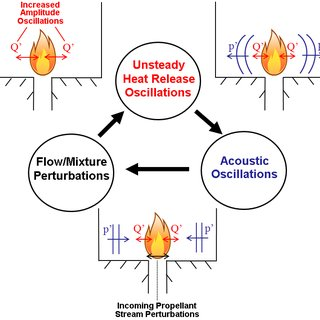
\includegraphics[width=0.4\textwidth]{./ti.jpg}
  \end{center}
  \caption{Thermoacoustic Instability}
 \label{fig:Thermoacoustic Instability}
\end{wrapfigure} 
Acoustic feedback or instability,refers to the phenomenon where the sound produced by an acoustic system (such as a guitar) is picked up by a microphone, amplified, and then played back through a loudspeaker. This creates a loop where the sound from the speaker is picked up again by the microphone, leading to a continuous and often loud howling sound. These  instabilities are caused from two sources, soundbox and string.\cite{Acoustic Instability}\\

\textit{Soundbox Instability} involves the sound propagating back towards the guitar's top plate, causing it to resonate and produce a disturbing feedback sound while feedback due to \textit{String Instability} can result in extended sustain or swelling of the string's vibration. While extended sustain is desirable, uncontrollable swelling of vibration can lead to loud, narrowband sounds if not managed properly. \\

Thermoacoustics is concerned with the interactions between heat (thermo) and pressure oscillations in gases (acoustics). Sound wave consists of compression (condensation) and expansion (rarefaction). At the area of compression a temperature rise occurs while at rarefaction occurs a temperature drop. These temperature oscillations accompany the pressure oscillations and they combine to produce the “Thermo-acoustic Effect”.\cite{Thermoacoustic Instability} 
%So thermoacoustic devices can convert temperature gradient to acoustic waves or convert acoustic waves to temperature gradient. When pressure waves are being created it is a thermoacoustic engine and when a temperature gradient is being created it is a thermoacoustic heat pump. Although in everyday life, the thermal effects of sound are too small, in a pressurized gas, these thermoacoustic effects can be used to create powerful heat engines and refrigerators. 

\section{Rijke's Tube}

Rijke's tube turns heat into sound, by creating a self-amplifying standing wave. It is basically an open-ended tube with a properly placed heat source inside.  Normally, the tube is positioned vertically and the heat source is introduced from below. Mean flow is caused either by natural convection (in vertical tubes) or by external means (in horizontal tubes).To study the thermoacoustic phenomenon, the apparatus was designed and constructed with the facility to change the heat source position and the heat input of the source.  Experiments were conducted by changing the heat input, heat source position, the tube length and diameter. Effects of these parameters on the output sound level were studied. \cite{Rijke Tube Article}

\subsection{Setup}
\begin{figure}[H] 
\centering
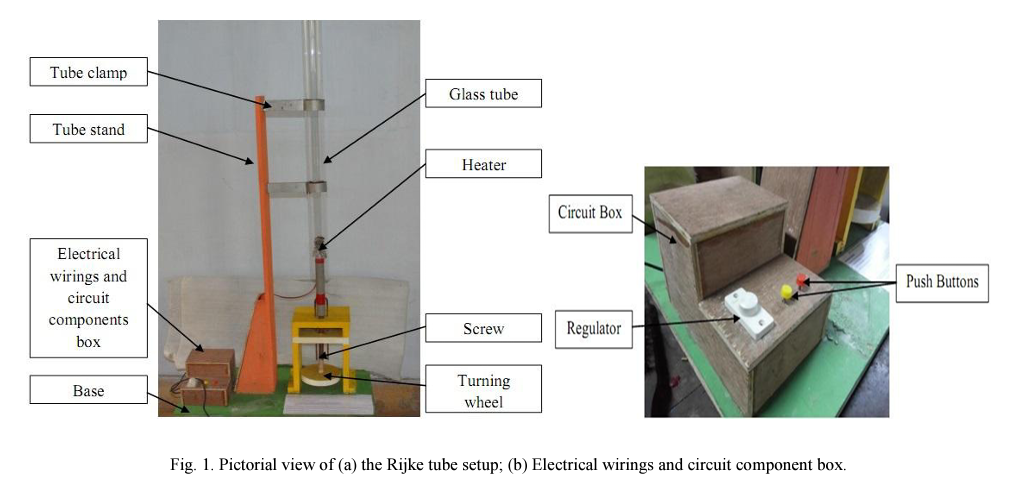
\includegraphics[width=0.9\columnwidth]{./rijketube.png}
\caption{Rijke Tube Apparatus}
\label{fig:Rijke Tube Apparatus}
\end{figure}

The experimental setup\cite{Rijke Tube Paper} consisted of a glass tube where a standing sound wave was generated, with a heater serving as the heat source to initiate and reinforce the sound. A screw mechanism allowed for vertical motion of the heater within the tube, facilitated by a wooden turning wheel. Electrical components, including a microcontroller and regulator, were housed in a circuit box to control the timing and intensity of current input. Measurements were taken for sound power, air temperature, and heater temperature at different current inputs to assess power output. Analysis revealed a discrepancy between the heat input and sound power output, highlighting the low efficiency of thermoacoustic devices.

Rijke initially proposed that a heat source at the tube's lower end created upward airflow by heating the air, causing it to rise and become denser upon contact with the cooler upper half of the tube, leading to compression and expansion cycles. However, this explanation lacked completeness. Lord Rayleigh's theory suggested that heat addition during compression and heat removal during expansion sustained acoustic waves.\\\\
Rayleigh criterion is used to determine the stability of a combustion system based on the phase relationship between pressure and heat release rate fluctuations. \cite{CI in LRE}
\begin{equation}
    \int_{0}^{L} \frac{\left( \gamma - 1 \right)}{\rho c^{2}} Q' p' dx > \left(p' u' A \right)_{L} - \left(p' u' A \right)_{0}
\end{equation}
where,
\begin{center}
L is the length of the system or domain, 0 is the lower limit of integration,\\
$\gamma$ is the ratio of specific heats,\\
$\rho$ is the density of the fluid,\\
$c$ is the speed of sound in the fluid,\\
$Q_{0}$ is a characteristic flow rate,\\
$p_{0}$ is the characteristic pressure,\\
$u_{0}$ is the characteristic velocity,\\
$A$ is the characteristic area.\\
\end{center}
Two conclusions can be reached from Rayleigh’s criterion: 
\begin{enumerate}
	\item Acoustic perturbations are enhanced when the total energy gained through unsteady combustion is larger than the total energy dissipated through the system boundaries.
	\item Energy of the acoustic perturbations is increased when the rate of unsteady heat release is in phase with the pressure oscillations. Thus, if the unsteady heat release rate is of a large enough amplitude, with the phase offset between the acoustic pressure oscillations and the unsteady heat release rate being approximately zero (at least $|φ_{o}| < 90^{o}$), growth of the instability is promoted.
\end{enumerate}
The heat transfer was divided into mean and time-varying components, where mean transfer induced convective flow, and time-varying transfer drove the acoustic wave. Heat addition during compression and removal during expansion sustained the wave. Placing the source midway maximized sound output since it balanced heat transfer effects on pressure. This detailed understanding elucidates the complex interplay of heat transfer and acoustic wave dynamics in the Rijke tube phenomenon.\cite{Rijke Tube Paper}

\begin{figure}[H] 
\centering
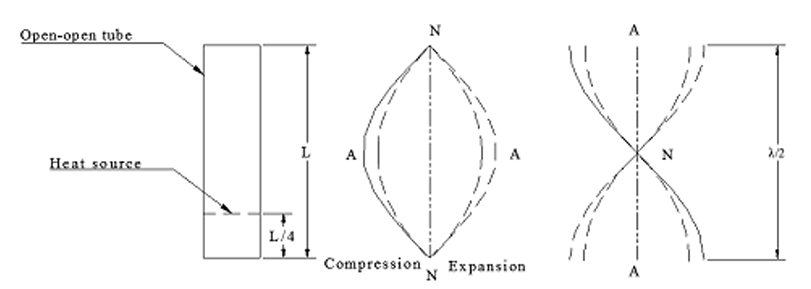
\includegraphics[width=0.6\columnwidth]{./rijketheory.png}
\caption{Pressure oscillation and velocity (change of displacement) oscillations in Rijke tube}
\label{fig:Pressure oscillation and velocity (change of displacement) oscillations in Rijke tube}
\end{figure}
 

\subsection{Discussion}

The experimental findings provided insights into the relationship between various parameters such as current, heater temperature, tube dimensions, and heater position on sound generation in a Rijke tube setup, contributing to a better understanding of thermoacoustic phenomena and the efficiency of thermoacoustic devices.\cite{Rijke Tube Paper}
\begin{itemize}
\item \textbf{Variation of Air Temperature and Sound Level with Current and Heater Temperature} - Increasing the current through the coil led to higher air temperature and sound level due to more heating in the system. This resulted in greater reinforcement of the standing wave and increased sound intensity.
\item \textbf{Effect of Tube Length and Diameter} - Tube length and diameter had a significant impact on sound generation. There was an optimal tube length for maximum sound output, and changes in diameter affected the heating of the air inside the tube, influencing sound generation.
\item \textbf{Position of Heater and Sound Power Output} - The position of the heater inside the tube influenced the sound level, with an optimal position (one quarter of the length from the bottom end) for highest sound output. The calculated sound power output was low compared to the heat input, indicating the inefficiencies of thermoacoustic devices.
\item \textbf{Input Power and Sound Level} - Sound level increased with input current and power, but there was a threshold value below which sound generation did not occur due to inadequate heating. The position of the heater inside the tube also played a role in sound output.
\end{itemize}

\subsection{Conclusion}
In conclusion, the study on thermoacoustic phenomenon in a Rijke tube provided valuable insights into the complex interplay between heat and pressure oscillations, as demonstrated through sound generation in the experimental setup. By aligning with Rayleigh's estimation on the optimal position of the heater, the research not only validated theoretical principles but also underscored the practical implications for enhancing thermoacoustic device efficiency.\\
The study explores the mechanisms behind sound generation in Rijke tubes, highlighting the importance of understanding and controlling thermoacoustic phenomena for optimizing engine performance and stability, paving the way for further exploration into mitigating combustion instabilities.

\section{V2 Rocket}
The V2 was the first ballistic guided missile with advanced rocket technology and was used in WWII by the Nazi’s against the Allies. It was a liquid propellant rocket engine of liquid ethanol (which took 30 tons of potatoes to fuel a single launch) and liquid oxygen. The final V2 design weighed 12,500 kg, was 14 m in length and 1.65 m in diameter.The A4 incorporated four major advances - its powerful engine, its aerodynamic shape, its innovative guidance system and its radio transmission system.\cite{V2 Rocket}
\begin{figure}[H] 
\centering
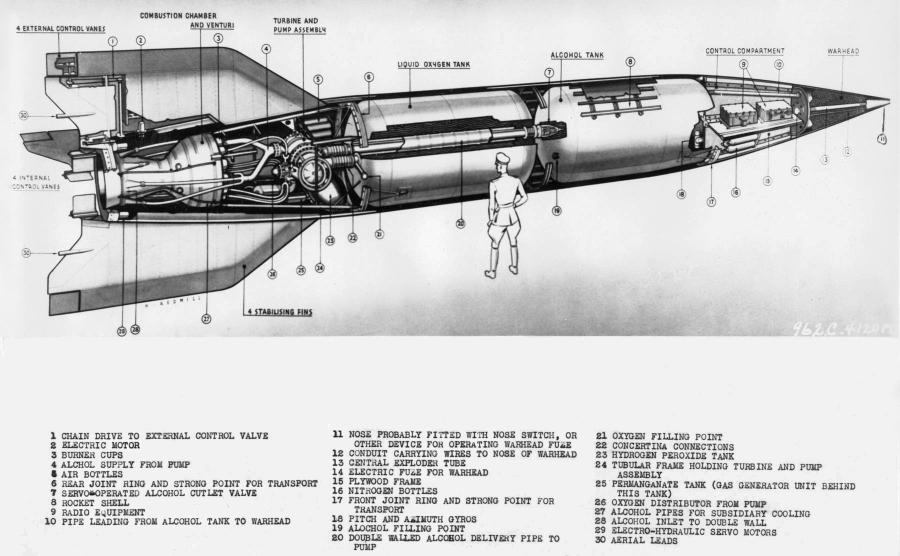
\includegraphics[width=0.5\columnwidth]{./v2rocket.jpg}
\caption{Parts of V2 Rocket}
\label{fig:v2rocket}
\end{figure}
\begin{itemize}
\item The engine introduced a new fuel nozzle for watered alcohol injection, allowing better atomization and efficient combustion. A pre-chamber system combined propellant and oxidizer in small compartments above the main combustion chamber, preventing heat damage to nozzles and enhancing fuel mixing.
\item Secondly, the aerodynamic shape of the rocket was a big concern since it would be travelling very fast, particularly the fins would help control it. 
\item Third, the V2 had an inertial guidance system and used four vanes in the middle of the rocket exhaust to deflect thrust to steer the rocket. This was unlike any other rockets developed before.
\item The final advance was the development of a radio transmission system that could relay information about the missile's performance to the ground.
\end{itemize}

\subsection{Issues with V2 Engine}
During the course of the rocket firings, the underlying reasons for issues were identified. Despite their seemingly minor nature, these issues had significant consequences. The first identified problem was a dropping relay, attributable to resonance vibrations. The second issue pertained to the loosening of fittings within the propellant pipelines, a consequence of vibrations and a vulnerability in the design and structure of the outer skin at the ogival forward section. Upon re-entry into the atmosphere, the outer skin, already weakened by the heat generated from air friction, exhibited fluttering. This fluttering exacerbated the skin's compromised integrity, leading to a temperature rise of approximately $6000^{\circ}$ Celsius. Ultimately, the compromised skin ruptured, allowing air ingress, culminating in the missile's disintegration.\cite{The German V2}
\subsection{Conclusion}
The work on this engine proved to be the inspiration to build launch vehicles used in the upcoming space race.  It is regarded as a revolutionary breakthrough in rocket technology, with the use of liquid fuel increasing its thrust capabilities and making it the first artificial object to enter space.
%Chapman-Jouguet Condition: The Chapman-Jouguet condition defines the minimum conditions required for a detonation wave to propagate in a combustible mixture.  
%dVdP =V1 (1−γ1​ ) where:P is the pressure,V is the volume,γ is the specific heat ratio.
%Combustion Efficiency: The combustion efficiency equation quantifies the effectiveness of the combustion process in converting the chemical energy of propellants into thermal energy. η 
%c =Q˙fuel Q˙released​ where:ηc​  is the combustion efficiency,Q˙released​  is the rate of heat release,Q˙fuel​  is the rate of fuel energy input.

\section{Titan II Engine}
The Titan II rocket engine played a crucial role in the Gemini project, which was a manned spaceflight program conducted by NASA during the mid-1960s. The Titan II was a two-stage liquid-fuel rocket. The first stage was powered by an LR87 engine (with two combustion chambers and nozzles, fed by separate sets of turbomachinery), and the second stage was propelled by an LR-91 engine, was used to launch the Gemini spacecraft, which carried astronauts into space to conduct various missions and experiments.\cite{Titan II GLV}\\
The Gemini project aimed to develop and test various spaceflight capabilities essential for the Apollo program, which had the ultimate goal of landing astronauts on the Moon. The Gemini missions focused on tasks such as spacewalks, orbital maneuvers, rendezvous and docking procedures, and long-duration spaceflights.
\subsection{Setup}
\begin{wrapfigure}{r}{0.6\textwidth}
  \begin{center}
    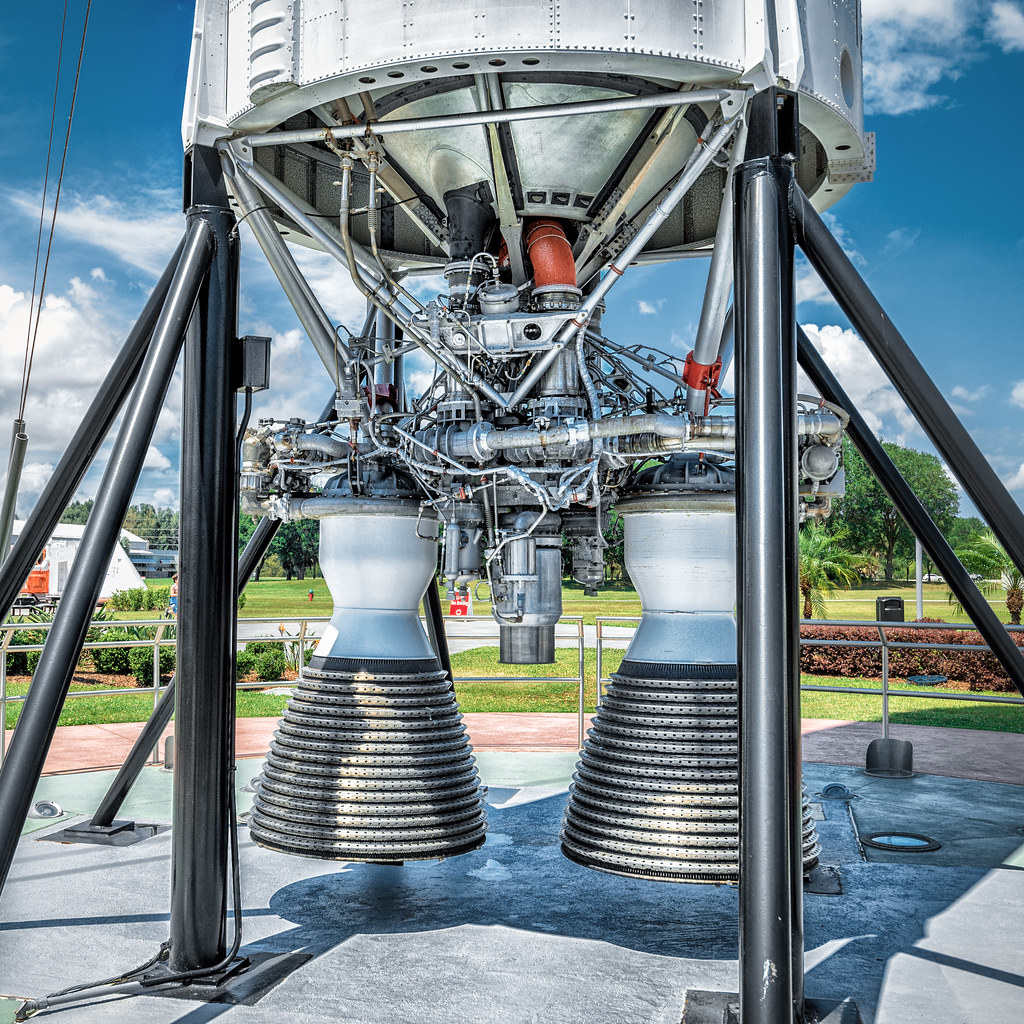
\includegraphics[width=0.4\textwidth]{./titanII.jpg}
  \end{center}
  \caption{Titan II Gemini Launch Vehicle}
  \label{fig:titanII}
\end{wrapfigure}
The Titan II rocket engine, a vital component of the Titan II GLV, featured a sophisticated setup designed for reliable and efficient propulsion during space missions, including the Gemini project. The engine utilized hypergolic propellants, Aerozine 50 (a mixture of hydrazine and unsymmetrical dimethylhydrazine) as fuel, and nitrogen tetroxide as the oxidizer, known for their ignition upon contact.

Within the thrust chamber, these propellants underwent combustion, generating high-pressure, high-temperature gases expelled through the rocket nozzle to produce thrust. An ignition system ensured timely and reliable engine start-up, crucial for successful launches. To prevent overheating, the engine incorporated regenerative cooling, circulating propellants around the thrust chamber to absorb heat and maintain structural integrity. A gimbal system allowed controlled movement of the engine nozzle, providing thrust vector control for trajectory adjustments during flight. Thrust vector control mechanisms enabled precise steering and stabilization, adjusting thrust direction for pitch, yaw, and roll control.

The robust thrust structure supported the engine and transmitted thrust to the rocket, designed to withstand high forces and vibrations during launch and flight. Integrated into the Titan II launch vehicle, the engine's performance and reliability were essential for mission success. Overall, the Titan II engine's setup combined advanced propulsion technology, ignition systems, cooling mechanisms, thrust vector control, and structural support to deliver efficient and dependable rocket propulsion for space exploration missions like the Gemini project.

\subsection{Discussion}
The Titan II rocket engine, a pivotal component of the Titan II launch vehicle, played a crucial role in various space missions, including the Gemini project. While the engine demonstrated significant capabilities, it also faced several challenges and problems during its operational history. 
One of the notable issues with the Titan II engine was related to its hypergolic propellants, Aerozine 50 and nitrogen tetroxide. These propellants, while efficient in generating thrust upon contact, posed safety concerns due to their toxic and corrosive nature. Handling and storage of these propellants required stringent safety protocols to prevent accidents and ensure the well-being of personnel working with the engine.\\
\begin{wrapfigure}{r}{0.5\textwidth}
  \begin{center}
    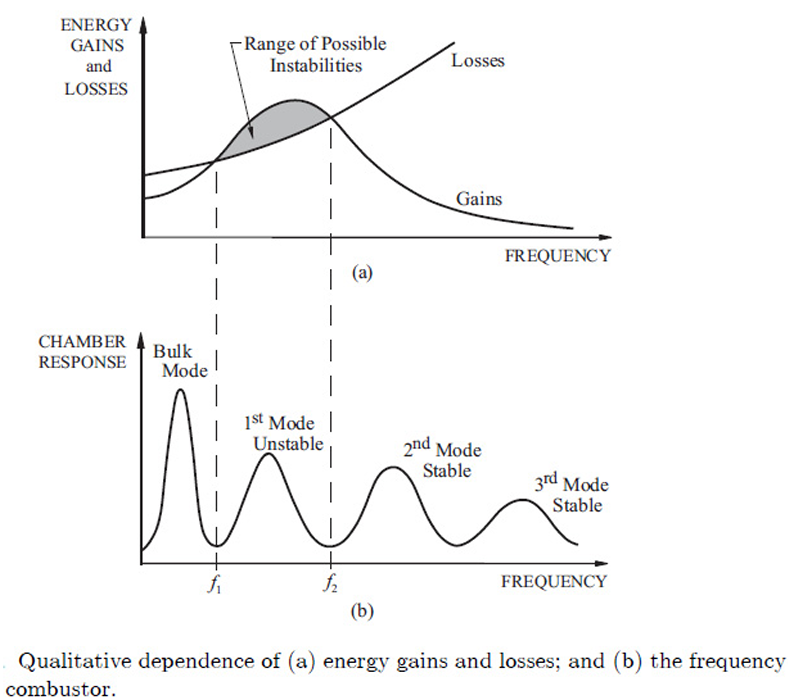
\includegraphics[width=0.5\textwidth]{./lpe_freq.png}
  \end{center}
 \caption{Combustion Instability }
\label{fig:lpe_freq}
\end{wrapfigure} 
Another challenge encountered by the Titan II engine was related to its combustion stability. Combustion instabilities, characterized by pressure oscillations and fluctuations during the combustion process, could lead to performance issues, structural vibrations, and potential engine failure. Managing and controlling combustion instabilities required advanced design techniques and mitigation strategies to ensure the engine's reliability and performance.\cite{Space Launch Vehicle Complexity}\\\\
Combustion instabilities in liquid rocket engines can be categorized into high and low-frequency modes, each with distinct characteristics and underlying mechanisms that contribute to instability. Understanding the theory behind these pressure fluctuations is crucial for developing effective control strategies to mitigate combustion instabilities.\\High-frequency combustion instabilities typically refer to pressure oscillations with frequencies in the kilohertz range. These instabilities are often associated with the interaction between the unsteady heat release from combustion and the acoustic properties of the combustion chamber. The rapid energy release from combustion can excite acoustic modes (longitudinal modes in the Titan II engine)\cite{CI in LRE}  within the chamber, leading to pressure fluctuations at high frequencies. The coupling between the heat release rate and acoustic waves can create a positive feedback loop, amplifying the instabilities.
%\begin{figure}[H] 
%\centering
%\includegraphics[width=0.5\columnwidth]{./longitudinal.jpg}
%\caption{Longitudinal Instability}
%\label{fig:Longitudinal Instability}
%\end{figure}
\\On the other hand, low-frequency combustion instabilities involve pressure oscillations at lower frequencies, typically in the range of a few hertz to a few hundred hertz. These instabilities are often linked to the dynamics of the combustion process itself, including fuel injection, mixing, and combustion efficiency. Variations in fuel-air mixing, flame propagation, and combustion stability can lead to periodic pressure fluctuations at lower frequencies. These low frequency instability modes is contributed to “POGO” instabilitie\cite{POGO}
\begin{figure}[H] 
\centering
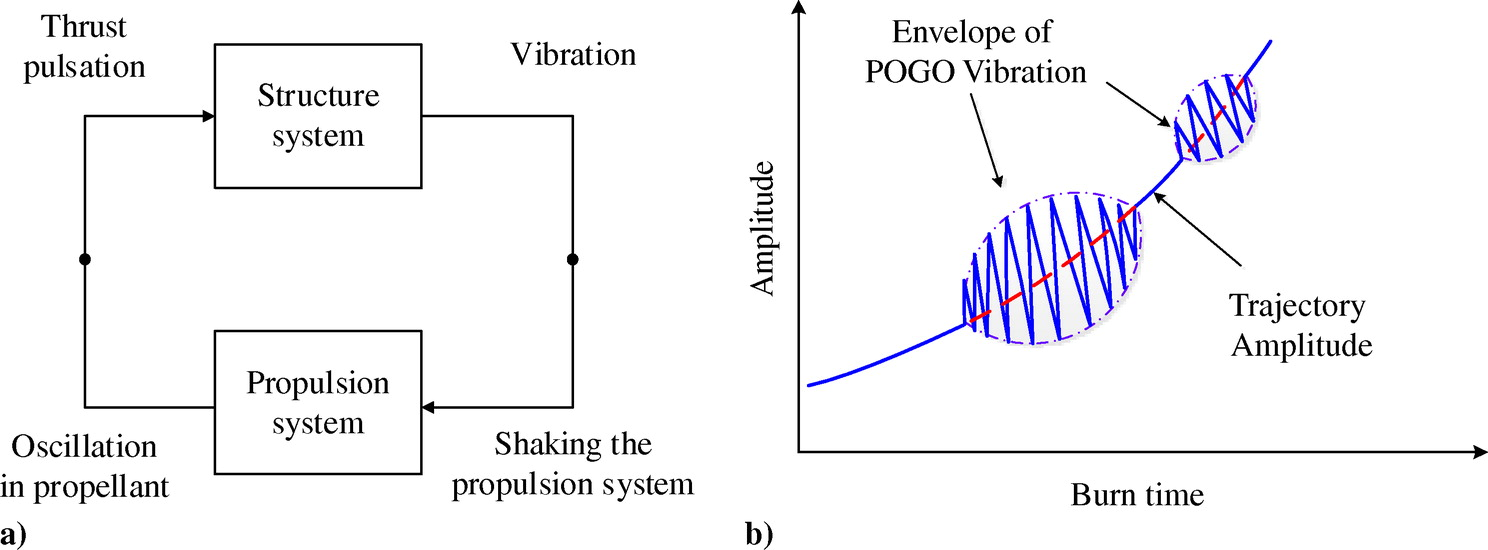
\includegraphics[width=0.8\columnwidth]{./pogo.jpeg}
\caption{ POGO Instability}
\label{fig:POGO Instability}
\end{figure}

The theory behind high and low-pressure frequency fluctuations causing combustion instability underscores the complex interplay between combustion dynamics, acoustic properties of the chamber, and the feedback mechanisms that govern instability growth. Effective control techniques for addressing these instabilities may involve modifying injector designs, optimizing fuel-air mixing, adjusting chamber geometry, or implementing active control strategies such as acoustic excitation or fuel modulation to dampen pressure oscillations and stabilize combustion.
By gaining a deeper understanding of the theoretical foundations behind high and low-pressure frequency fluctuations in combustion instabilities, engineers can develop targeted approaches to enhance the stability and performance of liquid rocket engines, ensuring safe and reliable operation during space missions.\\\\
Additionally, the Titan II engine faced issues with thrust vector control and engine gimbal mechanisms. Precise control of the engine nozzle for thrust vectoring and trajectory adjustments was essential for accurate flight dynamics. Any malfunctions or inaccuracies in the thrust vector control system could impact the rocket's stability and trajectory during ascent, potentially jeopardizing mission success.
Despite these challenges, the Titan II engine's engineering advancements and capabilities contributed significantly to space exploration missions. Continuous improvements and refinements in design, safety protocols, and operational procedures helped address and mitigate the problems encountered, enhancing the engine's performance and reliability over time.


\subsection{Conclusion}
Combustion instability, caused by oscillatory flow patterns, affects the energy release rate in engines. Early experiments show that transverse velocity components play a big role, especially near the injector face. Baffles in chambers disrupt these patterns, reducing velocity oscillations based on blade length and spacing.\cite{CI in LRE of NASA}  Detailed studies on baffle effects are limited, but experiments on Gemini launch vehicle engines suggest increasing blade numbers or spacing enhances stability. The goal is to minimize combustion gain across all modes; if not possible, damping via baffles or resonators is necessary. Different injector types exhibit varied stability characteristics, with some requiring baffles for stabilization.\\\\
%The Titan II rocket engine, with its reliability and performance, played a significant role in the success of the Gemini project by ensuring the safe and efficient launch of astronauts into space.
The combination of the Titan II rocket engine and the Gemini spacecraft paved the way for advancements in space exploration and laid the foundation for the Apollo missions that followed.
Overall, the Titan II engine's role in the Gemini project exemplifies the importance of reliable propulsion systems in enabling human spaceflight and advancing our understanding of space exploration.

\section{Summary}
We immerse ourselves in the captivating world of Thermoacoustic Instability in aerospace propulsion, showcasing the intricate interplay between heat transfer and acoustic dynamics. Through a lens that spans from Rijke's Tube to the V2 Rocket and the Titan II Engine, we are drawn into a narrative that blends science, history, and engineering. Rijke's Tube serves as a starting point, illustrating the conversion of heat into sound waves through self-amplifying standing waves. Moving beyond, the V2 Rocket emerges as a symbol of innovation during WWII, with its advanced engine design and guidance system fueled by liquid ethanol and oxygen. Transitioning to the Titan II Engine, we glimpse the future of space exploration, highlighting the ongoing quest for stability in combustion processes. By exploring parameters like current input, tube dimensions, and heater position, the study offers insights into optimizing sound generation and efficiency in thermoacoustic devices. This report weaves together past achievements, present challenges, and future aspirations in aerospace propulsion, painting a dynamic portrait of the evolving landscape of propulsion technology.

\newpage
\section{Bibliography}
\begin{thebibliography}{99}

\bibitem{Acoustic Instability}
Feedback Control in an Actuated Acoustic Guitar Using Frequency Shifting\\ \url{https://research.aalto.fi/files/34665627/ELEC_Thuillier_Feedback_Control_JAES.pdf}

\bibitem{Thermoacoustic Instability}
Chapter 7 -\emph{Thermoacoustic Instability}- Xiaofeng Sun, Xiaoyu Wang\\ \url{https://www.sciencedirect.com/science/article/pii/B9780124080690000075/pdfft?md5=753ca085ef1a9fa9b96c66f9e07f1b4f&pid=3-s2.0-B9780124080690000075-main.pdf}

\bibitem{Rijke Tube Paper}
\emph{Study of Thermoacoustic phenomenon in a Rijke tube} - C. A. A. Atis*, M. Sarker, M. Ehsan\\ \url{https://www.sciencedirect.com/science/article/pii/S1877705814028963/pdf?md5=d3cc90647cfa9b6103e4920674251f2c&pid=1-s2.0-S1877705814028963-main.pdf}

\bibitem{Rijke Tube Article}
\emph{Rijke Tube - A Thermoacoustic Device} - Shekhar M Sarpotdar, N Ananthkrishnan and S D Sharma\\ \url{https://link.springer.com/content/pdf/10.1007/BF02834451.pdf}

\bibitem{Rijke Tube Video}
\emph{Rijke Tube Phenomenon Video}\\ \url{https://youtu.be/pncG3lJUOdY?feature=shared}

\bibitem{V2 Rocket}
\emph{The V2 Rocket} - War Memorial Blog\\ \url{https://www.awm.gov.au/articles/blog/v2rocket#:~:text=It%20was%20powered%20by%20a,chamber%20by%20two%20rotary%20pumps.
}

\bibitem{The German V2}
\emph{The German V-2} - Journal Article\\ \url{https://doi.org/10.2307/3101376}

\bibitem{Titan II GLV}
Titan II GLV Wiki\\ \url{https://en.wikipedia.org/wiki/Titan_II_GLV}

\bibitem{Space Launch Vehicle Complexity}
\emph{Understanding Space Launch Vehicle Complexity: A Case Study in Combustion Instabilities} - Ronald H. Freeman, PhD Candidate*\\ \url{https://www.sciencedirect.com/science/article/pii/S1877050915029725/pdf?md5=31941d7a8795c6a4dd9ed549c3b20471&pid=1-s2.0-S1877050915029725-main.pdf}

\bibitem{CI in LRE}
\emph{Overview of Combustion Instabilities in Liquid Rocket Engines - Coupling Mechanisms \& Control Techniques} - John W. Bennewitz∗ and Robert A. Frederick†\\ \url{https://www.researchgate.net/publication/268472794_Overview_of_Combustion_Instabilities_in_Liquid_Rocket_Engines_-_Coupling_Mechanisms_Control_Techniques}

\bibitem{POGO}
\emph{Enhanced Method for Analyzing Pogo Stability of Liquid Rockets with Uncertain-But-Bounded Parameters} - Tao Wang, Qian Ding, Ye Tang and Zhi-Sai Ma\\ \url{https://arc.aiaa.org/doi/full/10.2514/1.A35064}

\bibitem{CI in LRE of NASA} 
\emph{“Liquid Propellant Rocket Combustion Instability,”} Technical Report NASA SP-194, National Aeronautics \& Space Administration, Washington D.C., 1972 - Harrje, D. T. and Reardon, F. H.\\ \url{https://ntrs.nasa.gov/api/citations/19720026079/downloads/19720026079.pdf}
\end{thebibliography}


\end{document}